\documentclass{beamer} 
%\title{text}
%\author{text}
%\date{date}
\usetheme{Boadilla}

\usepackage{tikz}
\usetikzlibrary{mindmap,trees}
\usepackage{verbatim}
\usepackage{adjustbox}

\begin{document}

\begin{frame}{MINDMAP}
\begin{adjustbox}{max totalsize={.9\textwidth}{.7\textheight},center}
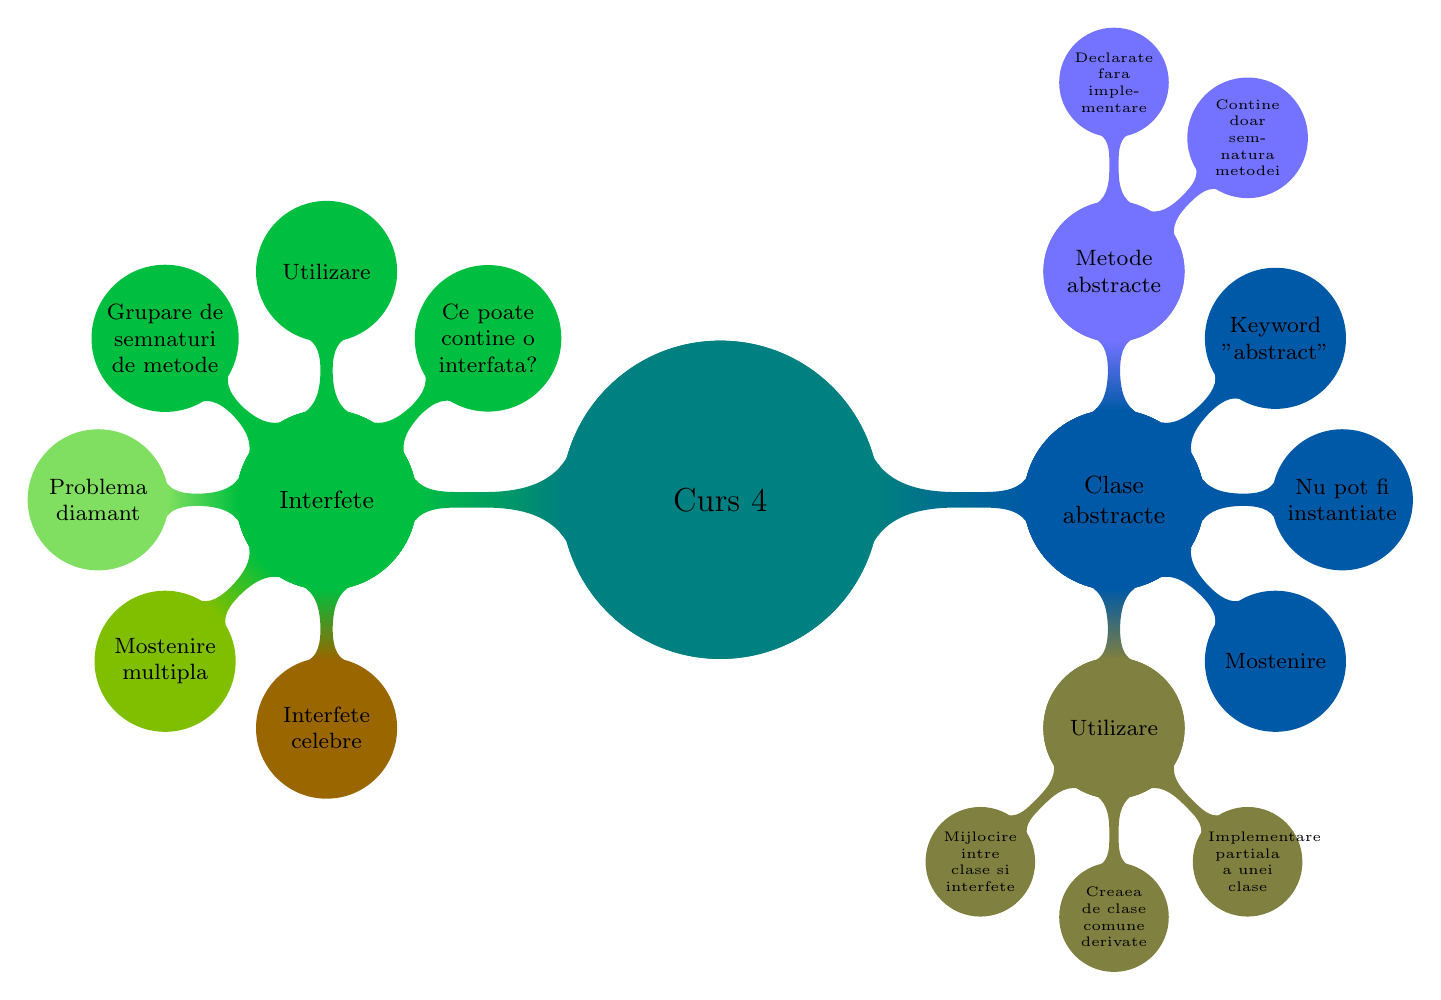
\begin{tikzpicture}
 	\path[mindmap, concept color=teal,text=black]
	node[concept] {Curs 4} [clockwise from=0]
	child[concept color = blue!30!teal] {
		node[concept] {Clase abstracte} [clockwise from=90] 
			child[concept color = white!45!blue]{
				node[concept] {Metode abstracte}[clockwise from=90] {child{node[concept]{Declarate fara implementare}}}
				node[concept] {Metode abstracte}[clockwise from=45] {child{node[concept]{Contine doar semnatura metodei}}}
}
		node[concept] {Clase abstracte} [clockwise from=45] 
			child[concept color = blue!30!teal]{node[concept] {Keyword "abstract"} }
		node[concept] {Clase abstracte} [clockwise from=-45] 
			child[concept color = blue!30!teal]{node[concept] {Mostenire} }
		node[concept] {Clase abstracte} [clockwise from=0] 
			child[concept color = blue!30!teal]{node[concept] {Nu pot fi instantiate} }
		node[concept] {Clase abstracte} [clockwise from=-90] 
			child[concept color = orange!50!teal]{
				node[concept]{Utilizare}[clockwise from = -90] {child{node[concept]{Creaea de clase comune derivate}}}
				node[concept]{Utilizare}[clockwise from = -45] {child{node[concept]{Implementare partiala a unei clase}}}
				node[concept]{Utilizare}[clockwise from = -135] {child{node[concept]{Mijlocire intre clase si interfete}}}
}
}
	node[concept] {Curs 4} [clockwise from=180]
	child[concept color = green!50!teal] {
		node[concept] {Interfete} [clockwise from=45] 
			child{node[concept] {Ce poate contine o interfata?} }	
		node[concept] {Interfete} [clockwise from=135] 
			child{node[concept] {Grupare de semnaturi de metode} }	
		node[concept] {Interfete} [clockwise from=90] 
			child{node[concept] {Utilizare} }
		node[concept] {Interfete} [clockwise from=270] 
			child[concept color = red!60!green]{node[concept] {Interfete celebre} }	
		node[concept] {Interfete} [clockwise from=225] 
			child[concept color = orange!50!green]{node[concept] {Mostenire multipla} }
		node[concept] {Interfete} [clockwise from=180] 
			child[concept color = pink!50!green]{node[concept] {Problema diamant} }
}
;
\end{tikzpicture}
\end{adjustbox}
\end{frame}
\end{document}

